% *********************************************************************
% © 2024–2026 Jeremy Sylvestre
%
% Permission is granted to copy, distribute and/or modify this document
% under the terms of the GNU Free Documentation License, Version 1.3 or
% any later version published by the Free Software Foundation; with no
% Invariant Sections, no Front-Cover Texts, and no Back-Cover Texts. A
% copy of the license is included in the appendix entitled “GNU Free
% Documentation License” that appears in the output document of this
% PreTeXt source code. All trademarks™ are the registered® marks of
% their respective owners.
%
% *********************************************************************

\newcommand*{\xmin}{-2.5}
\newcommand*{\xmax}{2.55}
\newcommand*{\ymin}{-0.5}
\newcommand*{\ymax}{0.5}

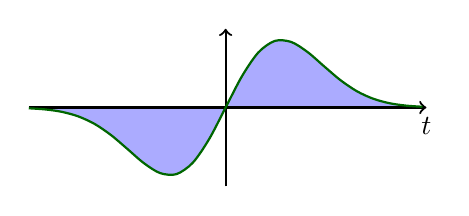
\begin{tikzpicture}[yscale=2]

	\fill[blue,opacity=0.33] plot[domain=0:2.5,smooth] (\x,{\x * exp(- \x * \x)}) -- (2.5,0) -- (0,0);
	\fill[blue,opacity=0.33] plot[domain=0:-2.5,smooth] (\x,{\x * exp(- \x * \x)}) -- (-2.5,0) -- (0,0);

	% axes
	\draw[->,thick] (\xmin,0) -- (\xmax,0) node[below] {$t$};
	\draw[->,thick] (0,\ymin) -- (0,\ymax);

	\draw[thick, green!40!black, domain=-2.5:2.5,smooth] plot (\x,{\x * exp(- \x * \x)});

\end{tikzpicture}
